\chapter{Résultats et analyse}

\section{Introduction}
Dans ce chapitre final nous allons analyser et discuter les résultats de l'application de l'ED. Les cas d'études considérés sont une cellule très largement étudiée dans la littérature et des module PV en mono-Si et poly-Si. On effectue aussi une analyse sur la stabilité et cohérence de la méthode avant de conclure avec une comparaison entre la méthode standard et le stratégie métaheuristique proposée à la fin du troisième chapitre. Tous les calculs effectués et les résultats on été obtenus avec \textit{Python 3.8.3} avec l'implementation standard \textit{CPython} et CPU \textit{Intel i5-7200U} avec une fréquence d'horloge maximale de 3.1\si{\giga\hertz} sous le système d'exploitation \textit{Arch Linux x86\_64} Kernel version \textit{5.7.2 arch1-1.}

\section{Cas d'études et résultats}
\subsection{Cas 1: Cellule 57-mm de RTC France}

Ce premier cas d'étude concerne la cellule en silicium de RTC France avec un diamètre de 57 mm qui a été très largement étudiée dans la littérature. Sa courbe caractéristique a été mesurée dans des conditions de température $T = \SI{33}{\celsius}$ et irradiance solaire $\SI{1000}{\watt\per\square\meter}$ et comprend 26 points expérimentaux (figure \ref{fig:RTCexp}). Figure \ref{fig:RTCres}.a montre que la caractéristique expérimentale et calculée par l'ED sont graphiquement quasi-identiques. Figure \ref{fig:RTCres}.b montre l'évolution de la moyenne des valeurs de fitness des vecteurs évalués par la fonction objectif dans chaque génération consécutive. On constate que dès la 50\textsuperscript{ème} génération, l'ED a pratiquement déjà convergé.

Le tableau \ref{tab:RTCres} présente une comparaison entre l'ED et d'autre méthodes appliquées à la cellule RTC France. On constate que les valeurs retrouvées par l'ED sont assez proches de celles des autres travaux. En effet, l'ED parvient à une erreur RMSE de \num{7.7692e-04} qui est supérieure aux autres techniques similaire comme les essaims particulaires \cite{Hamid2016}, l'algorithme des colonies d'abeilles artificielles \cite{Oliva2014} et l'ED à trois points \cite{Chin2019}. Les résultats les moins précis sont ceux de la méthode de Newton à moindres carrés \cite{Easwarakhanthan1986}.

\begin{table}[H]
  \caption{Bornes utilisées de l'espace de recherche pour le modèle simple diode}
  \label{tab:singleboundaries}

  \begin{center}
    \begin{tabular*}{\textwidth}{l@{\extracolsep{\fill}}lllll}
       \hline
       Paramètre         & $R_s$ & $R_{sh}$ & $a$ & $I_0$      & $I_{PV}$ \\
       \hline
       Borne supérieure  & 1     & 100      & 2   & \num{1e-06}& 10\\
       Borne inférieure  & 0     & 2        & 1   & \num{1e-07}& 0 \\
       \hline
    \end{tabular*}
  \end{center}
\end{table}

\begin{figure}[H]
  \begin{center}
    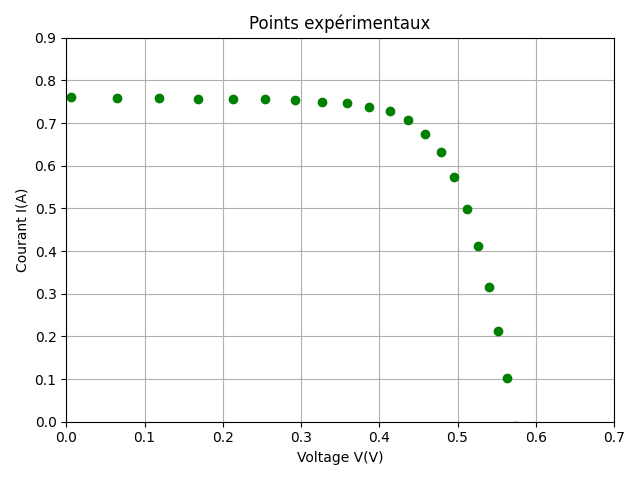
\includegraphics[width=0.5\textwidth]{resources/RTCFrance/exp.png}
    \caption{Données expérimentales de la caractéristique IV de la cellule RTC France mesurées à \SI{33}{\celsius}}
    \label{fig:RTCexp}
  \end{center}
\end{figure}

\begin{figure*}[h]
    \centering
    \begin{subfigure}[b]{0.45\textwidth}
        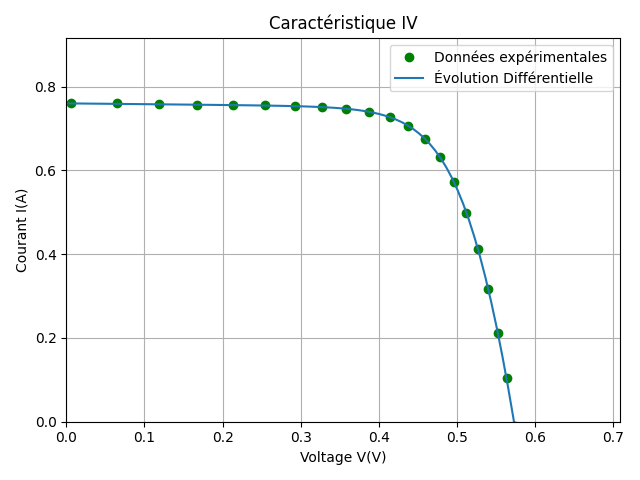
\includegraphics[width=\textwidth]{resources/RTCFrance/singled/iv.png}
        \caption{Comparaison entre la courbe expérimentale et la caractéristique calculée.}
    \end{subfigure}
    ~
    \begin{subfigure}[b]{0.45\textwidth}
        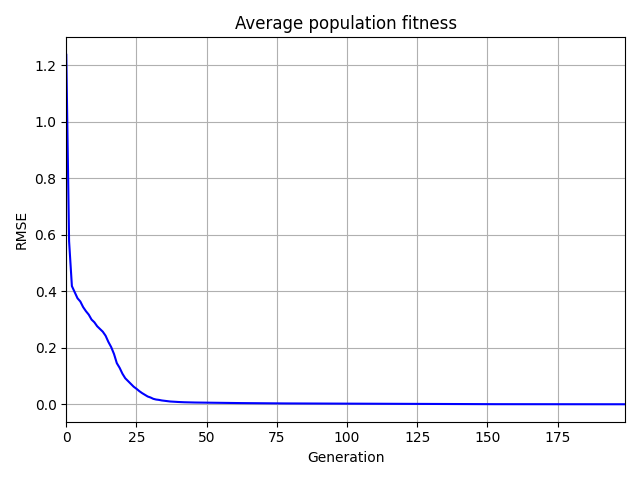
\includegraphics[width=\textwidth]{resources/RTCFrance/singled/fitness.png}
        \caption{Évolution de la valeur moyenne de fitness de chaque génération}
    \end{subfigure}
    \caption{Résultats de l'ED appliquée sur la cellule RTC France 57 mm.}
    \label{fig:RTCres}
\end{figure*}

\begin{table}[H]
  \caption{Comparaison de l'ED avec d'autres méthodes dans la littérature}
  \label{tab:RTCres}

  \begin{center}
  \scriptsize
    \begin{tabular*}{\textwidth}{l@{\extracolsep{\fill}}cllllll }
       \hline
       Paramètres & Référence & $R_s$ (\si{\ohm}) & $R_{sh} (\si{\ohm})$ & $a $ & $I_0$ (\si{\micro\ampere}) & $I_{PV}$ (\si{\ampere}) & $RMSE$ \\
       \hline
       ED (simple diode) &                            & \num{0.0363} & \num{54.1134} & \num{1.4709} & \num{0.3209} & \num{0.7607} & \num{7.7692e-04}\\
       ED3P              & \cite{Chin2019}            & \num{0.0363} & \num{54.1924} & \num{1.4798} & \num{0.3191} & \num{0.7607} & \num{8.1291e-04}\\
       PSO               & \cite{Hamid2016}           & \num{0.0363} & \num{53.8550} & \num{1.4816} & \num{0.3245} & \num{0.7607} & \num{9.8606e-04}\\
       ABC               & \cite{Oliva2014}           & \num{0.0364} & \num{53.6433} & \num{1.4817} & \num{0.3251} & \num{0.7608} & \num{9.8620e-04}\\
       Newton            & \cite{Easwarakhanthan1986} & \num{0.0364} & \num{53.7634} & \num{1.4837} & \num{0.3223} & \num{0.7608} & \num{9.70e-03}  \\
       GA                & \cite{Oliva2014}           & \num{0.0299} & \num{42.3729} & \num{1.5751} & \num{0.8087} & \num{0.7619} & \num{1.90e-02}  \\
       \hline
    \end{tabular*}
  \end{center}
\end{table}

\nomenclature{ED3P}{Évolution différentielle à trois points}
\nomenclature{ABC}{Colonies d'abeilles artificielles (\textit{Artificial Bee Colony Optimization})}

En ce qui concerne le modèle double diode, les deux facteurs d'idéalité $a_1$ et $a_2$ ainsi que les courants de saturation $I_{01}$ et $I_{02}$ sont indépendants les uns les autres mais sont contraints dans les limites dans le tableau \ref{tab:doubledboundaries}. Les résultats de l'ED en double diode sont comparés avec ceux de quelques autres méthode dans le tableau \ref{tab:RTCresdouble}.
\begin{table}[H]
  \caption{Bornes de l'espace de recherche à 7 dimensions}
  \label{tab:doubledboundaries}

  \begin{center}
  \small
    \begin{tabular*}{\textwidth}{l@{\extracolsep{\fill}}lllllll}
      \hline
      Paramètre & $R_s$ & $R_{sh}$ & $a_1$ & $a_2$ & $I_{01}$   & $I_{02}$    & $I_{PV}$ \\
      \hline
      Borne supérieure  & 1     & 100      & 2     & 2     & \num{1e-04}& \num{1e-04} & 10 \\
      Borne inférieure  & 0     & 2        & 1     & 1     & \num{1e-07}& \num{1e-07} & 0  \\
      \hline
    \end{tabular*}
  \end{center}
\end{table}

\begin{table}[H]
  \caption{Comparaison de l'ED avec d'autres méthodes dans la littérature}
  \label{tab:RTCresdouble}

  \begin{center}
  \scriptsize
    \begin{tabular*}{\textwidth}{l@{\extracolsep{\fill}}cllllllll}
       \hline
       Paramètres & Référence & $R_s$ (\si{\ohm}) & $R_{sh} (\si{\ohm})$ & $a_1$ & $a_2$ & $I_{01}$ (\si{\ampere}) & $I_{02}$ (\si{\ampere}) & $I_{PV}$ (\si{\ampere}) & $RMSE$ \\
       \hline
       ED (double diode) &                            & \num{0.02061}   & \num{51.9345} & \num{1.87579} & \num{1.43602} & \num{4.2322e-07} 
                                                      & \num{1.8726e-07}& \num{0.76055} & \num{7.63e-04}   \\
       ABC               & \cite{Oliva2014}           & \num{0.0364}    & \num{53.7804} & \num{1.4495} & \num{1.4885} & \num{4.07e-08}
                                                      & \num{2.874e-07} & \num{0.7608}  & \num{9.861e-04}\\
       PSO               & \cite{Jordehi2016}         & \num{0.05861}   & \num{18.2106} & \num{1.00012} & \num{1.00091} & \num{2.8601e-10} 
                                                      & \num{1e-12}     & \num{0.7633}  & \num{8.1646e-03} \\
       GSA               & \cite{Jordehi2017}         & \num{0.02914}   & \num{51.116}  & \num{1.6087}  & \num{1.62889} & \num{6.60621e-7} 
                                                      & \num{4.55149e-7}& \num{0.76886} & \num{5.91958e-03}\\
       \hline
    \end{tabular*}
  \end{center}
\end{table}

\nomenclature{GSA}{Gravitational Search Algorithm}

\subsection{Cas 2: Module monocristallin Schutten Solar STM6-40/36}

Nous nous concernons dans ce deuxième cas d'étude du module monocristallin Schutten Solar STM6-40/36 composé de 36 cellules ($156\si{\milli\meter}\times 156\si{\milli\meter}$) en série. Les données expérimentales ont été prises à une température de 51\si{\celsius}. Une comparaison des résultats de l'ED avec d'autres méthodes est présentée dans le tableau \ref{tab:stm6}. La correspondance de la caractéristique calculée par l'ED aux points experimentaux est démontrée graphiquement dans la figure \ref{fig:STM6res}. Malgré la distribution irrégulière des points, l'ED arrive a produire une solution précise. Sa précision et de même ordre de grandeur que ED3P \cite{Chin2019} mais elle est supérieure aux techniques des colonies des abeilles artificielles (ABC) \cite{Oliva2014}, de sa version améliorée par Oliva et al. (CIABC) \cite{Oliva2017a} et Chaotic Whale Optimization Algorithm (CWOA) \cite{Oliva2017}.

\begin{figure*}[t!]
    \centering
    \begin{subfigure}[b]{0.45\textwidth}
        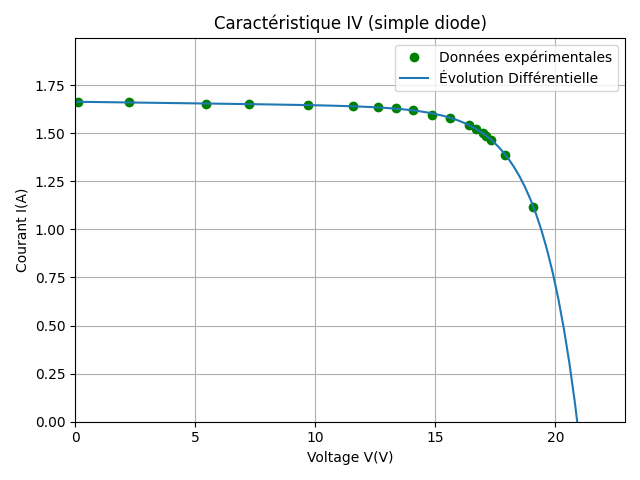
\includegraphics[width=\textwidth]{resources/STM6/singled/iv.png}
        \caption{Correspondence de l'ED aux données expérimentales. La distribution non-optimale des points n'entrave pas la convergence.}
    \end{subfigure}
    ~
    \begin{subfigure}[b]{0.45\textwidth}
        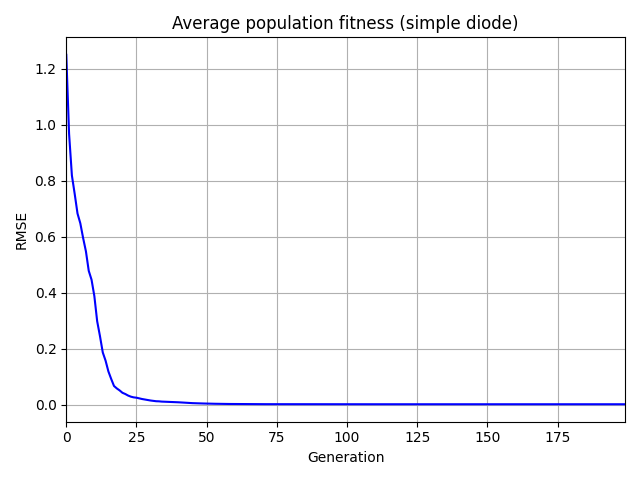
\includegraphics[width=\textwidth]{resources/STM6/singled/fitness.png}
        \caption{Évolution de la valeur moyenne de fitness de chaque génération. L'ED est convergeante dès la $50^{\text{ème}}$ itération.}
    \end{subfigure}
    \caption{Résultats de l'ED appliquée sur au module Schutten Solar STM6-40/36}
    \label{fig:STM6res}
\end{figure*}

\begin{table}[H]
  \caption{Comparaison de l'ED (simple diode) avec d'autres méthodes dans la littérature sur le module STM6-40/36}
  \label{tab:stm6}

  \begin{center}
    \scriptsize
    \begin{tabular*}{\textwidth}{l@{\extracolsep{\fill}}cllllll}
      \hline
      Paramètres & Référence & $R_s$ (\si{\milli\ohm}) & $R_{sh} (\si{\ohm})$ & $a $ & $I_0$ (\si{\micro\ampere}) & $I_{PV}$ (\si{\ampere}) & $RMSE$ \\
      \hline
       ED (simple diode)  &                   & \num{0.2801} & \num{16.5854} & \num{1.5571} & \num{2.8049} & \num{1.6633} & \num{1.7721e-03}  \\
       ED3P               & \cite{Chin2019}   & \num{0.4186} & \num{16.7328} & \num{1.5656} & \num{2.7698} & \num{1.6632} & \num{1.7740e-03}  \\
       ABC                & \cite{Oliva2014}  & \num{4.99}   & \num{15.206}  & \num{1.4866} & \num{1.5}    & \num{1.6644} & \num{1.838e-03}   \\
       CIABC              & \cite{Oliva2017a} & \num{4.4}    & \num{15.617}  & \num{1.4976} & \num{1.6642} & \num{1.6760} & \num{1.819e-03}   \\
       CWOA               & \cite{Oliva2017}  & \num{5}      & \num{15.4}    & \num{1.5}    & \num{1.6338} & \num{1.7}    & \num{1.800e-03}   \\
       \hline
    \end{tabular*}
  \end{center}
\end{table}
\nomenclature{CIABC}{Chaotic Improved Artificial Bee Colony}
\nomenclature{CWOA}{Chaotic Whale Optimization Algorithm}


Les résultats de l'ED avec le modèle double diode sur le module STM6-40/36 sont présenté dans le tableau \ref{tab:STM6double} avec d'autres techniques tel quel les colonies d'abeilles artificielles et les essaims particulaires. Le tableau \ref{tab:stm6doublelimits} montre les bornes utilisées comme limites de l'espace de recherche. Notons la similarité des qualités des résultats du modèle simple et double diode.

\begin{table}[H]
  \caption{Comparaison de l'ED (double diode) avec d'autres méthodes sur le module photovoltaïque STM6-40/36}
  \label{tab:STM6double}

  \begin{center}
  \scriptsize
    \begin{tabular*}{\textwidth}{l@{\extracolsep{\fill}}cllllllll}
       \hline
       Paramètres & Référence & $R_s$ (\si{\ohm}) & $R_{sh} (\si{\ohm})$ & $a_1$ & $a_2$ & $I_{01}$ (\si{\ampere}) & $I_{02}$ (\si{\ampere}) & $I_{PV}$ (\si{\ampere}) & $RMSE$ \\
       \hline
       ED (double diode) &                            & \num{0.0177}    & \num{16.7050}& \num{1.9049} & \num{1.52461}   & \num{1.006e-06} 
                                                      & \num{2.9858e-06}& \num{1.6633} & \num{1.7724e-03}   \\
       ELPSO             & \cite{RezaeeJordehi2018}   & \num{0.0138}    & \num{16.8580}& \num{1.8706} & \num{1.16648}   & \num{1.670e-08} 
                                                      & \num{6.21092e-6}& \num{1.6648} & \num{1.8307e-03}   \\
       ABC               & \cite{RezaeeJordehi2018}   & \num{0.03434}   & \num{26.0613}& \num{1.9851}  & \num{1.4687}** & \num{8.938e-6} 
                                                      & \num{1e-12}     & \num{1.66347}& \num{2.0538e-03}\\
       \hline
    \end{tabular*}
  \end{center}
\end{table}
\nomenclature{ELPSO}{Enhanced Leader Particle Swarm Optimization}

\begin{table}[H]
  \caption{Limites de l'espace de recherche pour l'ED double diode sur le module photovoltaïque STM6-40/36}
  \label{tab:stm6doublelimits}

  \begin{center}
    \begin{tabular*}{\textwidth}{l@{\extracolsep{\fill}}lllllll}
      \hline
      Paramètre         & $R_s$ & $R_{sh}$ & $a_1$ & $a_2$ & $I_{01}$   & $I_{02}$    & $I_{PV}$ \\
      \hline
      Borne Supérieure  & 1     & 100      & 2     & 2     & \num{1e-04}& \num{1e-04} & 10\\
      Borne inférieure  & 0     & 2        & 1     & 1     & 0          & 0           & 0\\
      \hline
    \end{tabular*}
  \end{center}
\end{table}

\subsection{Cas 3: Module polycristallin Photowatt-PWP 201}

Le 3\textsuperscript{ème} cas concerne le module polycristallin Photowatt-PWP 201 composé de 36 cellules en série. Les données expérimentales ont été prise dans des conditions d'irradiation de $1000 \si{\watt\per\square\meter}$ et une température de $T = 45 \si{\celsius}$. Le tableau \ref{tab:pwpsingle} compare les résultats obtenus par Évolution Différentielle contre d'autres méthodes dans la littérature. Les valeurs des paramètres simple diode retrouvée par l'ED sont très similaires aux autres, mais sont plus précises en termes de RMSE. Figure \ref{fig:pwpsingle} montre la courbe caractéristique calculée (a) et la courbe de convergence de l'ED (b). Les bornes de l'espace de recherche sont identiques à celle de la cellule RTC France (Tableau \ref{tab:singleboundaries}) sauf pour le courant de saturation qu'on limite à $\num{1e-7} \leq I_{0} \leq \num{1e-5}$. Le modèle double diode est plus précis que le modèle simple diode avec l'ED, mais ce dernier reste plus précis que les autres techniques similaires.

\begin{table}[H]
  \caption{Comparaison de l'ED avec d'autres méthodes dans la littérature sur le module Photowatt-PWP 201}
  \label{tab:pwpsingle}

  \begin{center}
    \scriptsize
    \begin{tabular*}{\textwidth}{l@{\extracolsep{\fill}}cllllll}
      \hline
      Paramètres & Référence & $R_s$ (\si{\milli\ohm}) & $R_{sh} (\si{\ohm})$ & $a $ & $I_0$ (\si{\micro\ampere}) & $I_{PV}$ (\si{\ampere}) & $RMSE$ \\
      \hline
       ED (simple diode)  &                   & \num{0.0343} & \num{22.8238} & \num{1.3139} & \num{2.6380} & \num{1.0314} & \num{2.0529e-03}  \\
       ED3P               & \cite{Chin2019}   & \num{0.0347} & \num{19.3720} & \num{1.3002} & \num{2.1247} & \num{1.0335} & \num{2.4227e-03}  \\
       ISCE               & \cite{Gao2018}    & \num{0.0333} & \num{27.2772} & \num{1.3512} & \num{3.4823} & \num{1.0305} & \num{2.4251e-03}  \\
       CIABC              & \cite{Wu2018}     & \num{0.0333} & \num{27.2772} & \num{1.3512} & \num{3.4822} & \num{1.0305} & \num{2.425e-03}   \\
       Newton     & \cite{Easwarakhanthan1986}& \num{0.0335} & \num{15.2625} & \num{1.3458} & \num{3.2876} & \num{1.0318} & \num{5.6010e-01}  \\
       \hline
    \end{tabular*}
  \end{center}
\end{table}

\begin{figure*}[b!]
    \centering
    \begin{subfigure}[b]{0.45\textwidth}
        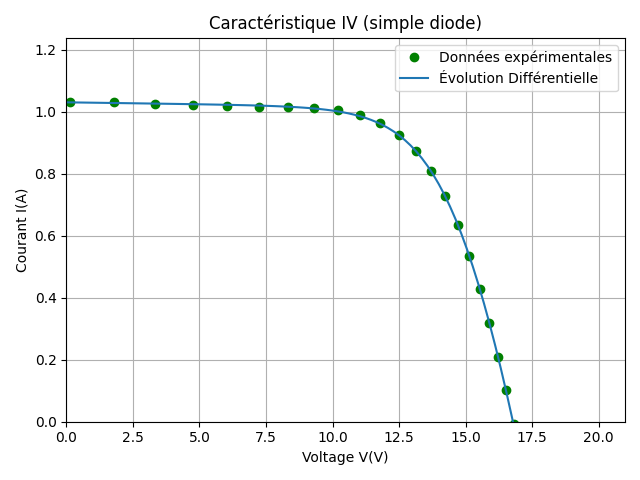
\includegraphics[width=\textwidth]{resources/pwp/iv.png}
        \caption{Caractéristique expérimentale et calculée du module polycristallin Photowatt-PWP 201.}
    \end{subfigure}
    ~
    \begin{subfigure}[b]{0.45\textwidth}
        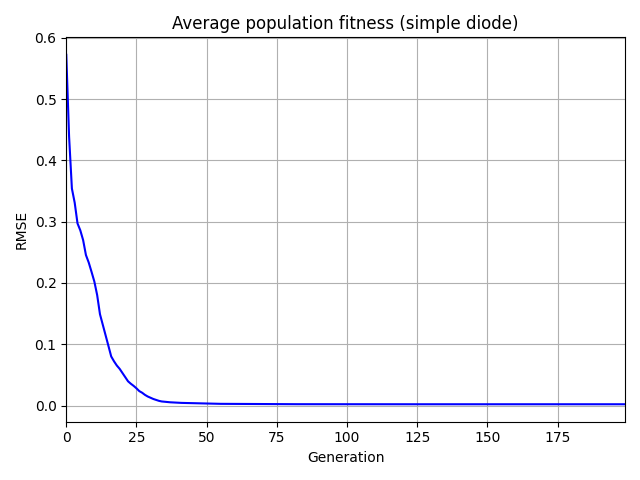
\includegraphics[width=\textwidth]{resources/pwp/fitness.png}
        \caption{Courbe de convergence de L'ED. Notons la convergence rapide (avant $< 100$ itérations)}
    \end{subfigure}
    \caption{Résultats de l'ED appliquée sur au module Photowatt PWP-201}
    \label{fig:pwpsingle}
\end{figure*}

\begin{table}[H]
  \caption{Comparaison de l'ED avec d'autres méthodes sur le module photovoltaïque Photowatt-PWP 201}
  \label{tab:pwpdouble}

  \begin{center}
  \scriptsize
    \begin{tabular*}{\textwidth}{l@{\extracolsep{\fill}}cllllllll}
       \hline
       Paramètres & Référence & $R_s$ (\si{\ohm}) & $R_{sh} (\si{\ohm})$ & $a_1$ & $a_2$ & $I_{01}$ (\si{\ampere}) & $I_{02}$ (\si{\ampere}) & $I_{PV}$ (\si{\ampere}) & $RMSE$ \\
       \hline
       ED (double diode) &                            & \num{0.8604}    & \num{19.2098}& \num{1.2165} & \num{1.5326}    & \num{1.6785e-7} 
                                                      & \num{2.6073e-06}& \num{1.03193}& \num{1.50208e-03}   \\
       TVACPSO           & \cite{Jordehi2016}         & \num{1.2356}    & \num{22.8236}& \num{1.3210} & \num{2.7778}   & \num{2.6381e-6} 
                                                      & \num{1e-12}     & \num{1.03143}& \num{2.0530e-03}   \\
       %ABC               & \cite{RezaeeJordehi2018}   & \num{0.03434}   & \num{26.0613}& \num{1.9851}  & \num{1.4687}** & \num{8.938e-6} 
       %                                               & \num{1e-12}     & \num{1.66347}& \num{2.0538e-03}\\
       \hline
    \end{tabular*}
  \end{center}
\end{table}

\subsection{Remarques}
Le modèle double diode contient deux termes exponentiels nécessitant deux évaluations de la fonction W de Lambert pour chaque point expérimental, ce qui est relativement coûteux d'un point de vue de calcul numérique. Par ailleurs, puisque tous les paramètres sont traités indépendamment des autres, l'espace de recherche est effectivement à 7 dimensions. Puisque la qualité des résultats des modèles simple et double diode est quasi-identique dans le cas de la cellule RTC France (Tableaux \ref{tab:RTCres} et \ref{tab:RTCresdouble} respectivement) ainsi que pour le module photovoltaïque monocristallin Schutten Solar STM6-40/36 (Tableaux \ref{tab:stm6} et \ref{tab:STM6double}), on constate que le modèle simple diode et très adéquat en terme de précision et supérieur en terme d'efficacité et rapidité de calcul.

\section{Analyse et cohérence de l'ED}

La performance supérieure démontrée par l'ED par rapport aux autres algorithmes provient probablement de ses capacités à la \textit{recherche globale}. L'existence d'une multitude de minimums locaux est démontrée dans la figure \ref{fig:neigh} où on a projeté l'espace de recherche 5-dimensionnel sur 2 dimensions au voisinage du minimum global. On fait varier le facteur d'idéalité $a$ et la résistance série $R_s$ dont le modèle est très sensible aux variations. Les trois autres paramètres $R_{sh}$, $I_0$ et $I_{PV}$ sont fixés sur les valeurs du minimum global retrouvé par l'ED comme dans le tableau \ref{tab:RTCres}.

\begin{figure}[H]
  \begin{center}
    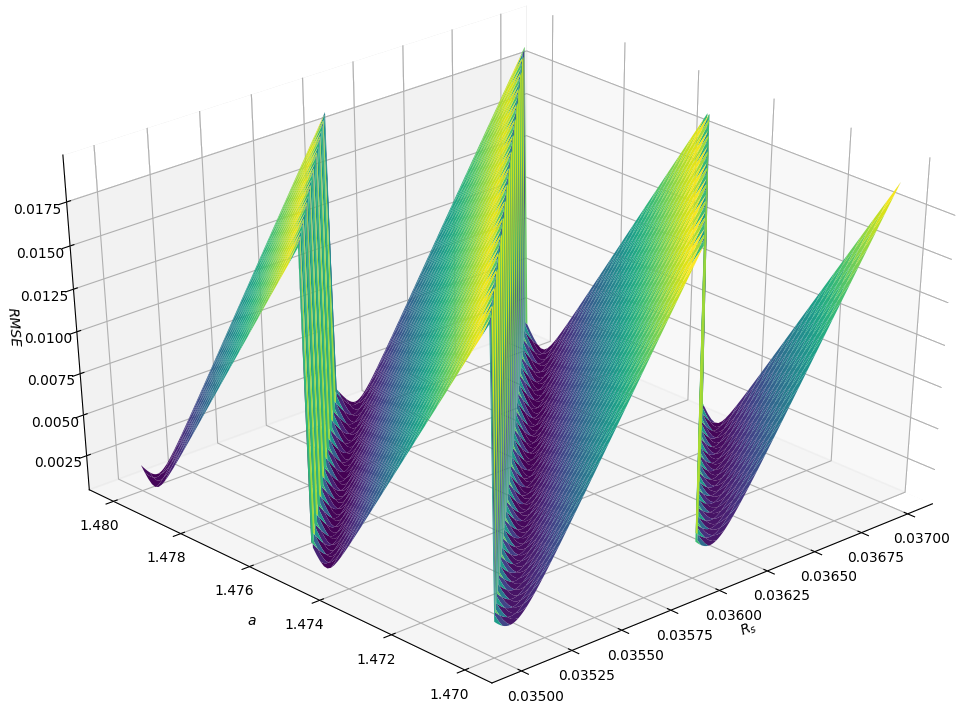
\includegraphics[width=0.75\textwidth]{resources/RTCFrance/singled/neighborhood.png}
    \caption{Le voisinage du minimum global retrouvé par l'ED selon le facteur d'idéalité et la résistance en série. Notons l'existence des "vallées" qui comprennent potentiellement plusieurs minimums locaux}
    \label{fig:neigh}
  \end{center}
\end{figure}

La nature stochastique de l'Évolution Différentielle fait qu'elle donne des résultats différents après chaque essai. Ceci impose une analyse de cohérence de la méthode pour estimer la fiabilité de l'ED pendant plusieurs essais consécutifs. Figure \ref{fig:consist} montre la RMSE de la solution finale dans 30 essais indépendants de l'ED.
Tous les points sont localisés dans une région très concentrée de l'espace de recherche ce qui indique que l'ED parvient effectivement à localiser le minimum global.
La cohérence des différents essais concernant la $R_s$ et le $a$ du module Photowatt-PWP 201 (Figure \ref{fig:paramconsist}) et les écart-types des paramètres montrés sur le tableau \ref{tab:RTCstats} confirment ceci puisque ils peuvent être interprétés comme un indice de "stabilité" de l'algorithme qui quantifié sa capacité a reproduire les mêmes résultats. Tous les écart-types sont de l'ordre de $10^{-3}$ ou moins, donc une solution précise est garantie dans n'importe quel essai.

\begin{figure*}
    \centering
    \begin{subfigure}[b]{0.45\textwidth}
        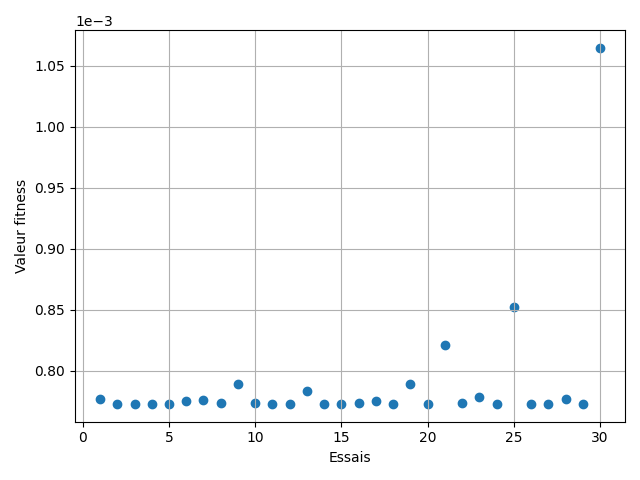
\includegraphics[width=\textwidth]{resources/RTCFrance/singled/consist.png}
        \caption{Cellule RTC France 57 mm}
    \end{subfigure}
    ~
    \begin{subfigure}[b]{0.45\textwidth}
        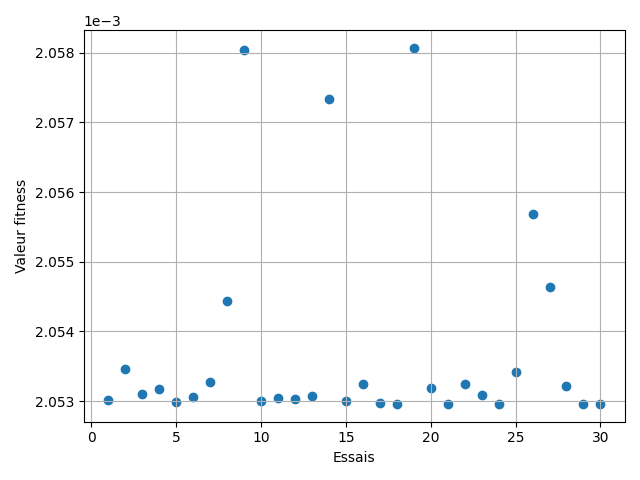
\includegraphics[width=\textwidth]{resources/pwp/consistency.png}
        \caption{Module Photowatt-PWP 201}
    \end{subfigure}
    \caption{Les RMSEs obtenues lors de 30 essais indépendants}
    \label{fig:consist}
\end{figure*}

\begin{figure*}
    \centering
    \begin{subfigure}[b]{0.45\textwidth}
        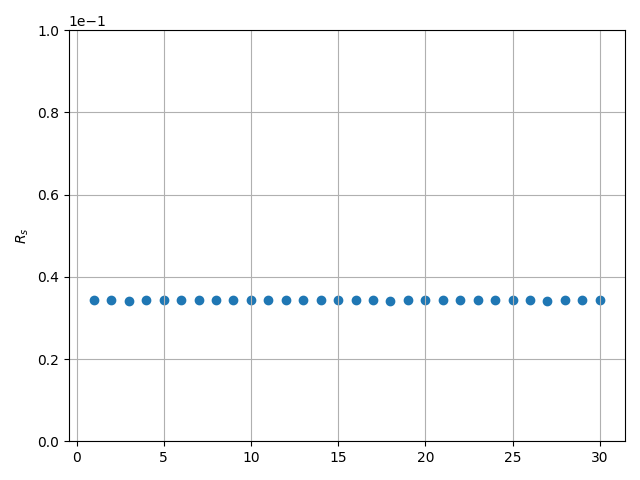
\includegraphics[width=\textwidth]{resources/pwp/rsconsist.png}
        \caption{Résistance série $R_s$}
    \end{subfigure}
    ~
    \begin{subfigure}[b]{0.45\textwidth}
        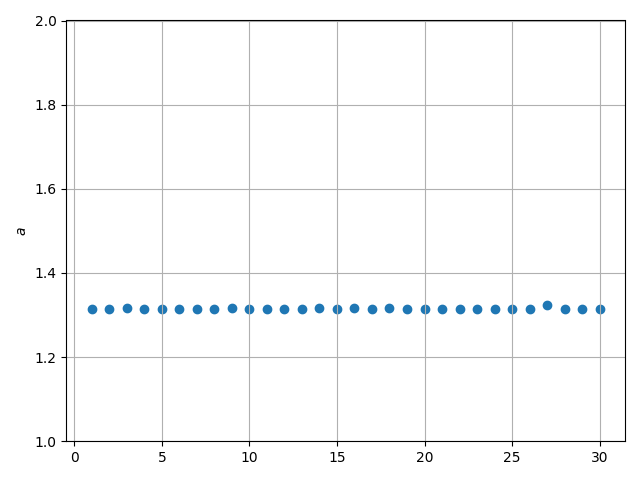
\includegraphics[width=\textwidth]{resources/pwp/aconsist.png}
        \caption{Facteur d'idéalité $a$}
    \end{subfigure}
    \caption{Résultats obtenus pour le facteur d'idéalité et la résistance série du module PHotowatt-PWP 201 pendant 30 essais indépendants}
    \label{fig:paramconsist}
\end{figure*}

\begin{table}
  \caption{Valeurs Moyennes de quelques paramètres influents de la cellule RTC France 57 mm et les écart-types associés des 30 essais}
  \label{tab:RTCstats}
  \small
  \begin{center}
    \begin{tabular*}{.7\textwidth}{c@{\extracolsep{\fill}}cc}
       \hline
       Paramètre & Valeur Moyenne & Écart-Type\\
       \hline
       $RMSE$       & \num{7.8925e-04}       & \num{5.3670e-05} \\
       $R_s$        & \num{3.6355e-02}       & \num{3.8936e-04} \\
       $a$          & \num{1.4722}           & \num{5.7539e-03} \\
       $I_0$        & \num{3.2655e-07}       & \num{3.4071e-08} \\
       \hline
    \end{tabular*}
  \end{center}
\end{table}

\section{Analyse de la stratégie métaheuristique}
Pour analyser la stratégie métaheuristique proposée dans le dernier chapitre, nous allons prendre le module polycristallin Photowatt-PWP 201.
Conformément aux recommandations de Storn et Price, nous avons choisi comme valeurs standard du facteur de mutation et du taux de croisement $0.7$ et $0.8$, respectivement. En fait les paramètres retrouvés dans le cas d'étude 3 avec les courbes caractéristique et de convergence, ont tous été retrouvé par l'ED configuré avec ces valeurs par défaut. Pour appliquer la métaheuristique, un nombre de population relativement faible est adéquat puisque notre espace de recherche est 2-dimensionnel: $N_P^{\text{higher order}} = 10 \times D = 20$. On limite aussi le nombre maximal de générations à $Gen_{max}^{\text{higher order}} = 50$. Pratiquement, la fonction objectif est donc la valeur fitness \textit{à la 50\textsuperscript{ème} itération}. Le fait que l'ED risque de pas avoir déjà converger ne nous pose pas de problèmes, puisque notre but est de retrouver les valeurs de $F$ et $CR$ permettant la convergence la plus rapide\footnote{Convergence rapide mais non-prematurée} que possible. Les paramètres de la métaheuristique elle-même sont $F^{\text{higher order}} = 0.8$ et $CR^{\text{higher order}} = 0.8$. 

Les résultats de cette stratégies pour le module Photowatt-PWP 201 sont:
\begin{equation}
  F = 0.55, \quad CR = 0.94
\end{equation}

Figure \ref{fig:metaconv} compare les courbes de convergences entre l'ED avec et sans stratégie métaheuristique. Malgré le fait que le facteur de mutation retrouvé est relativement plus bas que les recommandations de Storn et Price, il est toujours compris dans les limites de Zaharie et al. \cite{Zaharie2002}. Notons que la rapidité de convergence est sensiblement supérieure dans la figure \ref{fig:metaconv}.a, l'ED a déjà convergé à l'itération 25, alors que l'ED standard a besoin de deux fois plus d'itérations\footnote{Itérations et générations sont équivalentes dans ce cas}. En terme de temps de calcul, on teste dans le mêmes conditions les deux méthodes en les "chronométrant" avec Python. L'ED standard s'exécute au bout d'un temps moyen de $1.68535 \si{\second}$ sur 30 essais indépendants et un écart-type de $\num{4.751e-4}$. Pour l'ED avec métaheuristique, le temps moyen d'exécution est $0.82392 \si{\second}$, ce qui correspond à une diminution de 51\% du temps de calcul. Il n'y a pas de compromis envers la stabilité et la cohérence puisque l'écart-type des RMSEs est $\num{4.0162e-4}$. Figure \ref{fig:exectimes} montre les différents temps d'exécution pendant 30 essais avec les deux méthodes. Les valeurs initialement décroissantes sont probablement dues à l'utilisation des cache L1, et L2 du processeur.

\begin{figure*}
    \centering
    \begin{subfigure}[b]{0.45\textwidth}
        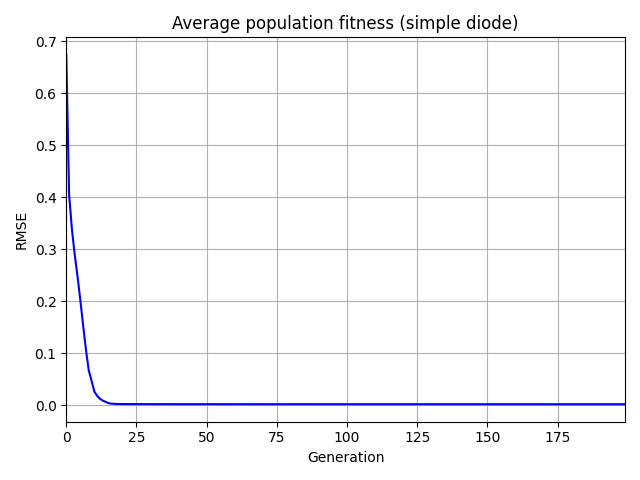
\includegraphics[width=\textwidth]{resources/pwp/metafit.png}
        \caption{Convergence de l'ED configurée avec les parametres retrouvée par la métaheuristique}
    \end{subfigure}
    ~
    \begin{subfigure}[b]{0.45\textwidth}
        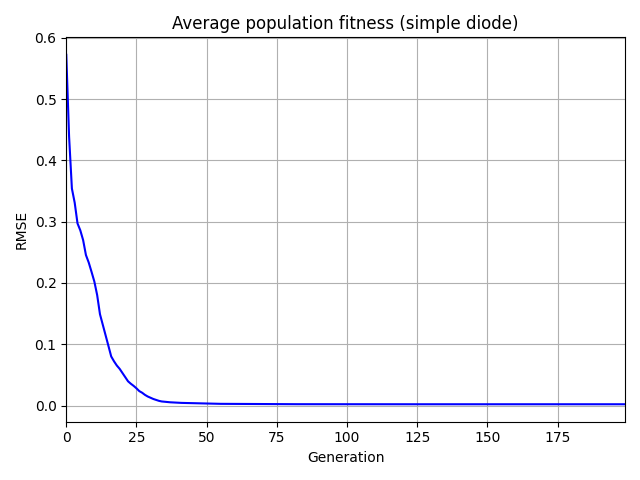
\includegraphics[width=\textwidth]{resources/pwp/fitness.png}
        \caption{Convergence de l'ED avec les paramètres standard}
    \end{subfigure}
    \caption{Comparaison de l'ED avec et sans métaheuristique}
    \label{fig:metaconv}
\end{figure*}

\begin{figure*}
    \centering
    \begin{subfigure}[b]{0.45\textwidth}
        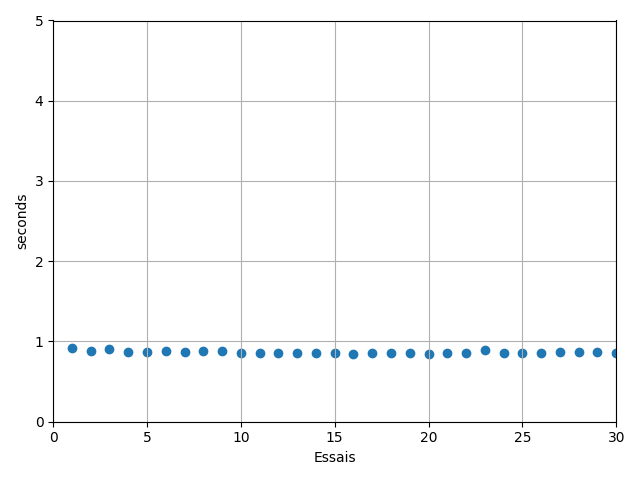
\includegraphics[width=\textwidth]{resources/metaexec.png}
        \caption{Avec stratégie métaheuristique}
    \end{subfigure}
    ~
    \begin{subfigure}[b]{0.45\textwidth}
        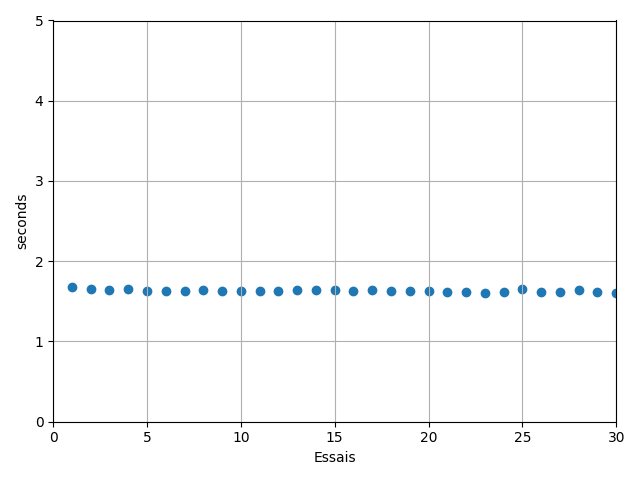
\includegraphics[width=\textwidth]{resources/stdexec.png}
        \caption{Avec ED standard}
    \end{subfigure}
    \caption{Comparaison des temps de calcul pendant 30 essais}
    \label{fig:exectimes}
\end{figure*}

\section{Conclusion}
